\documentclass{article}
\usepackage[utf8]{inputenc}

\usepackage{pgfplots}
\pgfplotsset{compat=1.18, width=10cm}

\title{1 -- Plotting}

\begin{document}
\maketitle

\section{Basic Plots}
\subsection{$f$ and $f'$}

\[
  f(x) = e^{-x} \sin(e^x)
\]
\[
  f'(x) = -e^{-x} \sin(e^x) + e^{-x} \cos(e^x) e^x
\]

Because we're discussing root-finding algorithms, let's plot $f$ and $f'$.

\subsubsection{png - matplotlib}

The standard method people usually use to plot in LaTeX.

\begin{figure}[h]
  \centering
  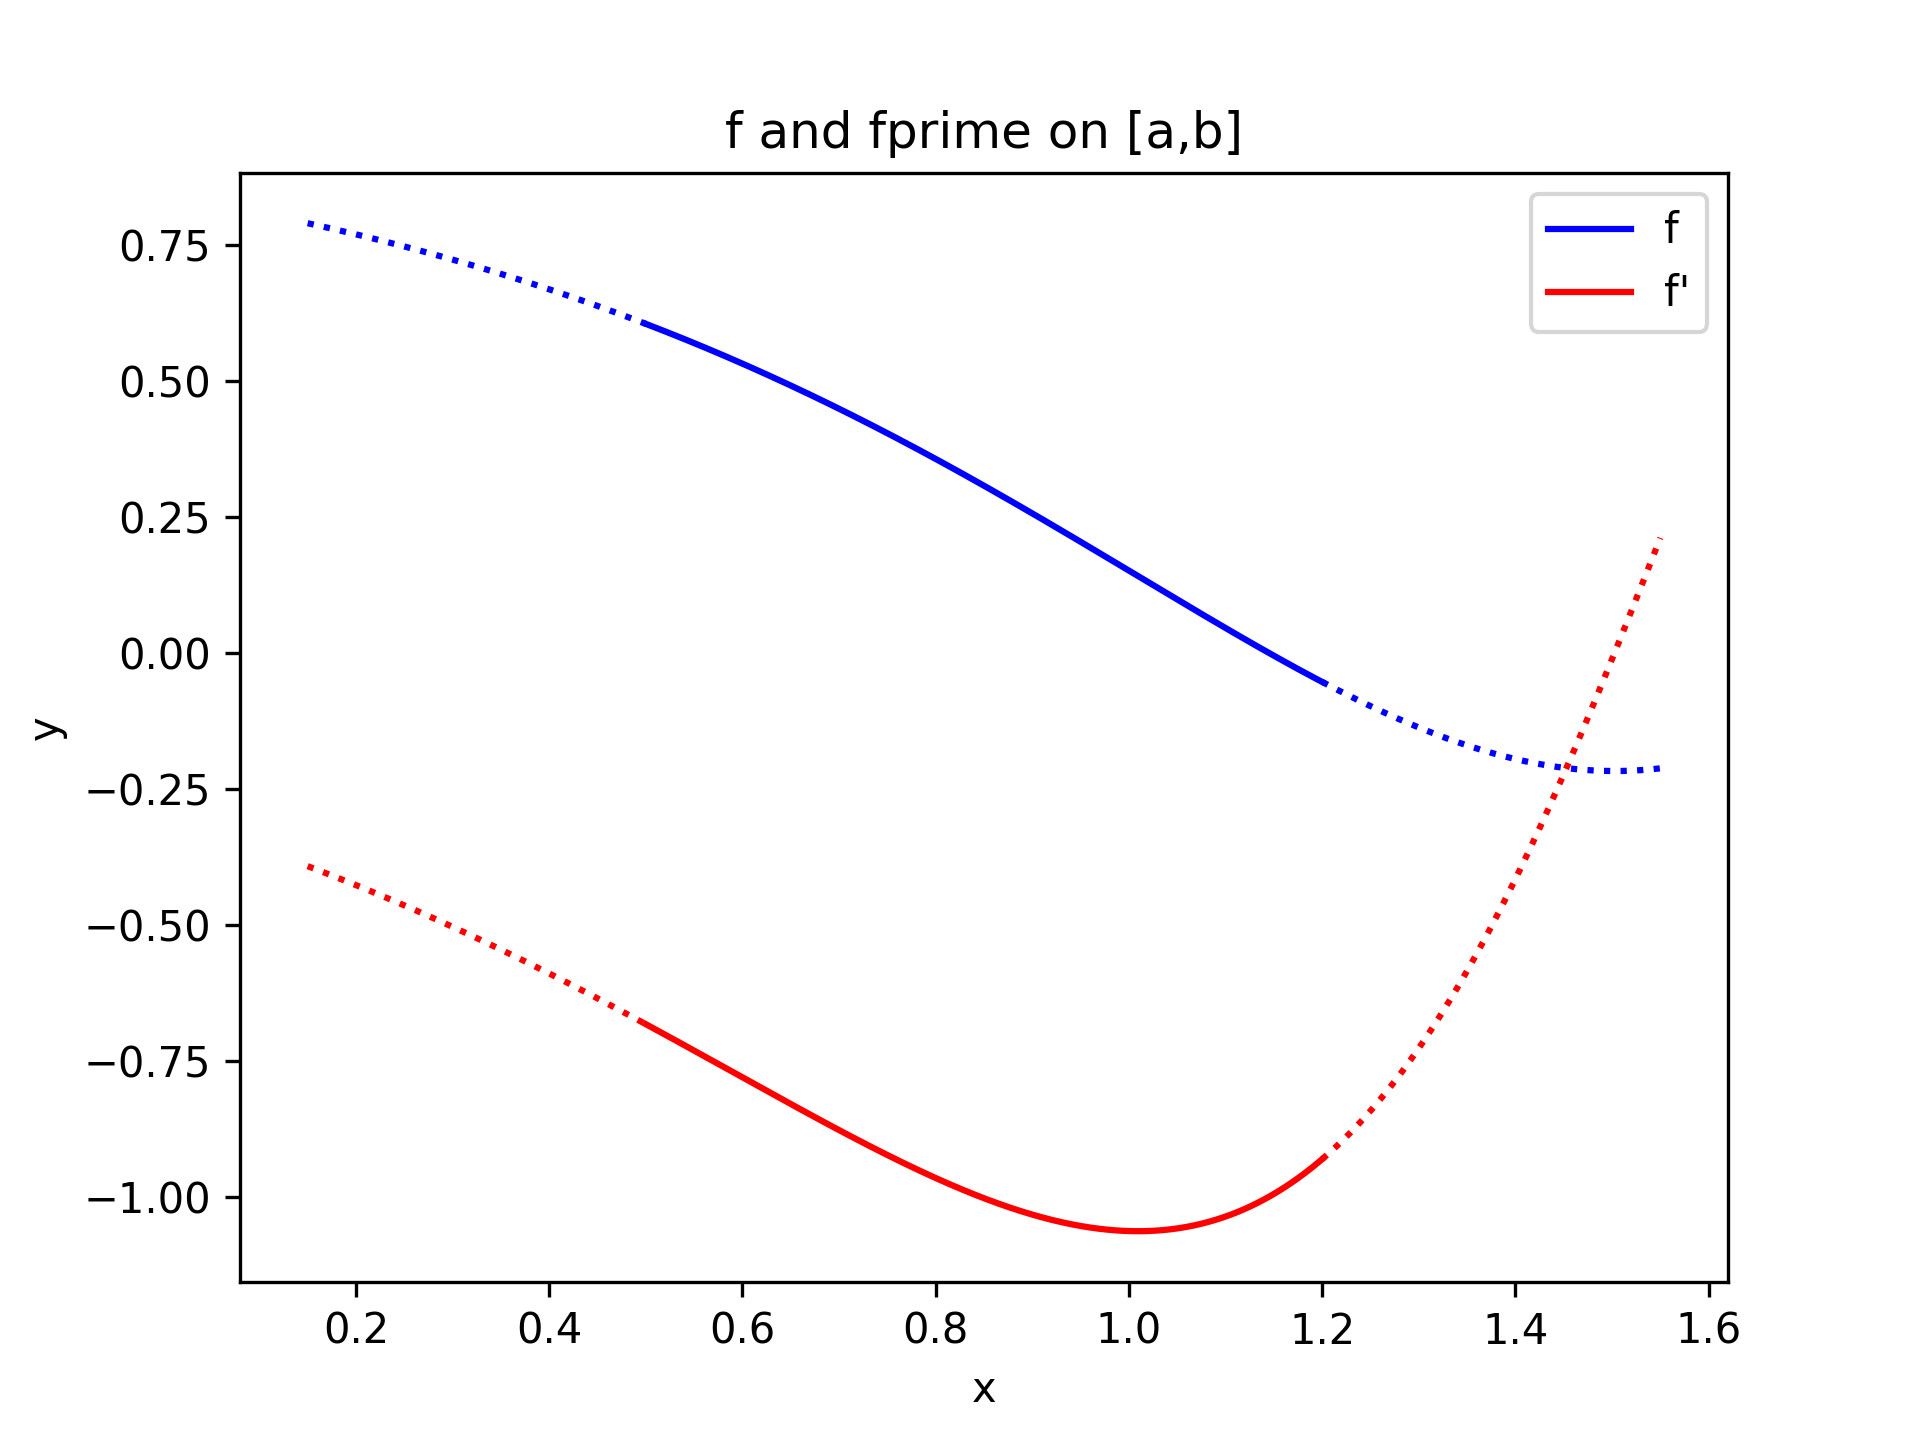
\includegraphics[scale=0.6]{./plots/ffp}
  \caption{A plot of $f$ and $f'$, $a = 0.5$ and $b = 1.2$}
\end{figure}

Notice how it looks a little off-center?
That's because the $y$-axis labels are long.
This will happen often when you do this.
You can play around with positioning, and size.


\subsubsection{svg - matplotlib}

\begin{figure}[h]
  \centering
  %\includesvg{./plots/svg/ffp.svg}
  \caption{An SVG plot of $f$ and $f'$, $a = 0.5$ and $b = 1.2$}
\end{figure}

Commented out, as Overleaf struggles with this.
You'd have to include the \texttt{svg} package in your preamble
and make sure \texttt{Inkscape} is installed and in your PATH.
Vector graphics do look good though, definitely an option.

\subsubsection{tikz - pgfplots}

This is a fun option. You can handcraft your plots in LaTeX
using the \texttt{tikz} package. This plot scales well when
zoomed in, and is very customizable. It can also be a lot of
work. 

\begin{figure}[h]
  \centering
    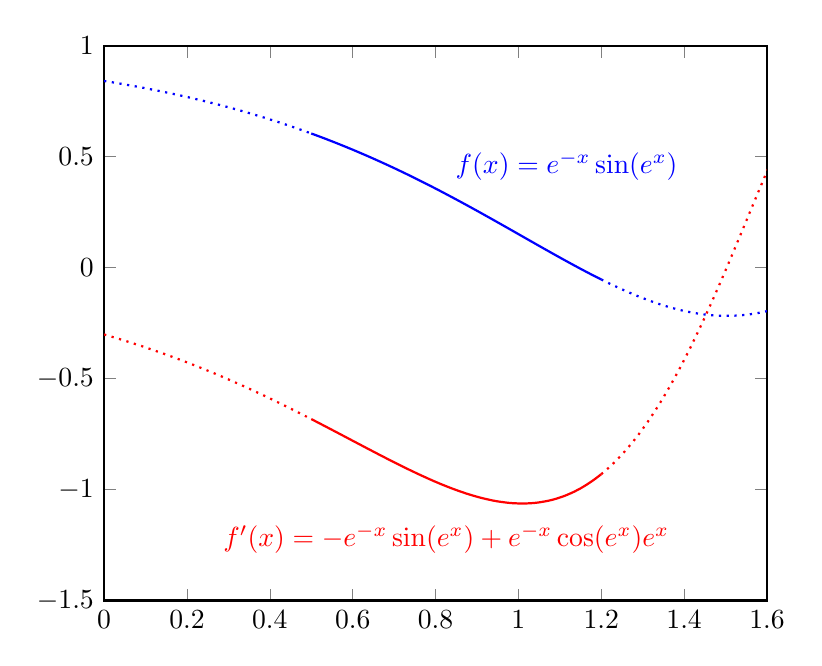
\begin{tikzpicture}
      \begin{axis}[
        samples=100,
        xmin=0, xmax=1.6,
        ymin=-1.5, ymax=1,
        axis lines=box,
        style=thick,
      ]
      \addplot[domain=0:0.5, color=blue, dotted]{e^(-x) * sin(deg(e^x))};
      \addplot[domain=0.5:1.2, color=blue]{e^(-x) * sin(deg(e^x))}
      node[right=20, pos=0.25]{$f(x) = e^{-x} \sin(e^x)$};
      \addplot[domain=1.2:2, color=blue, dotted]{e^(-x) * sin(deg(e^x))};
      
      \addplot[domain=0:0.5, color=red, dotted]{-1 * e^(-x) * sin(deg(e^x)) + e^(-x) * cos(deg(e^x)) * e^x};
      \addplot[domain=0.5:1.2, color=red]{-1 * e^(-x) * sin(deg(e^x)) + e^(-x) * cos(deg(e^x)) * e^x}
      node[below=10, pos=0.5]{$f'(x) = -e^{-x} \sin(e^x) + e^{-x} \cos(e^x) e^x$};
      \addplot[domain=1.2:2, color=red, dotted]{-1 * e^(-x) * sin(deg(e^x)) + e^(-x) * cos(deg(e^x)) * e^x};
      \end{axis}
    \end{tikzpicture}
  \caption{A TikZ plot of $f$ and $f'$}
\end{figure}


\newpage
\subsection{$f$ and its root}

Let's pick a specific root, $x=\ln(\pi)$ to target. What does this function
look like on a larger interval? Knowing the behavior of the function globally
helps inform why this might be challenging.

\subsubsection{png - matplotlib}

A plot of the root we're targeting with our three root-finding algorithms.


\begin{figure}[h]
  \centering
  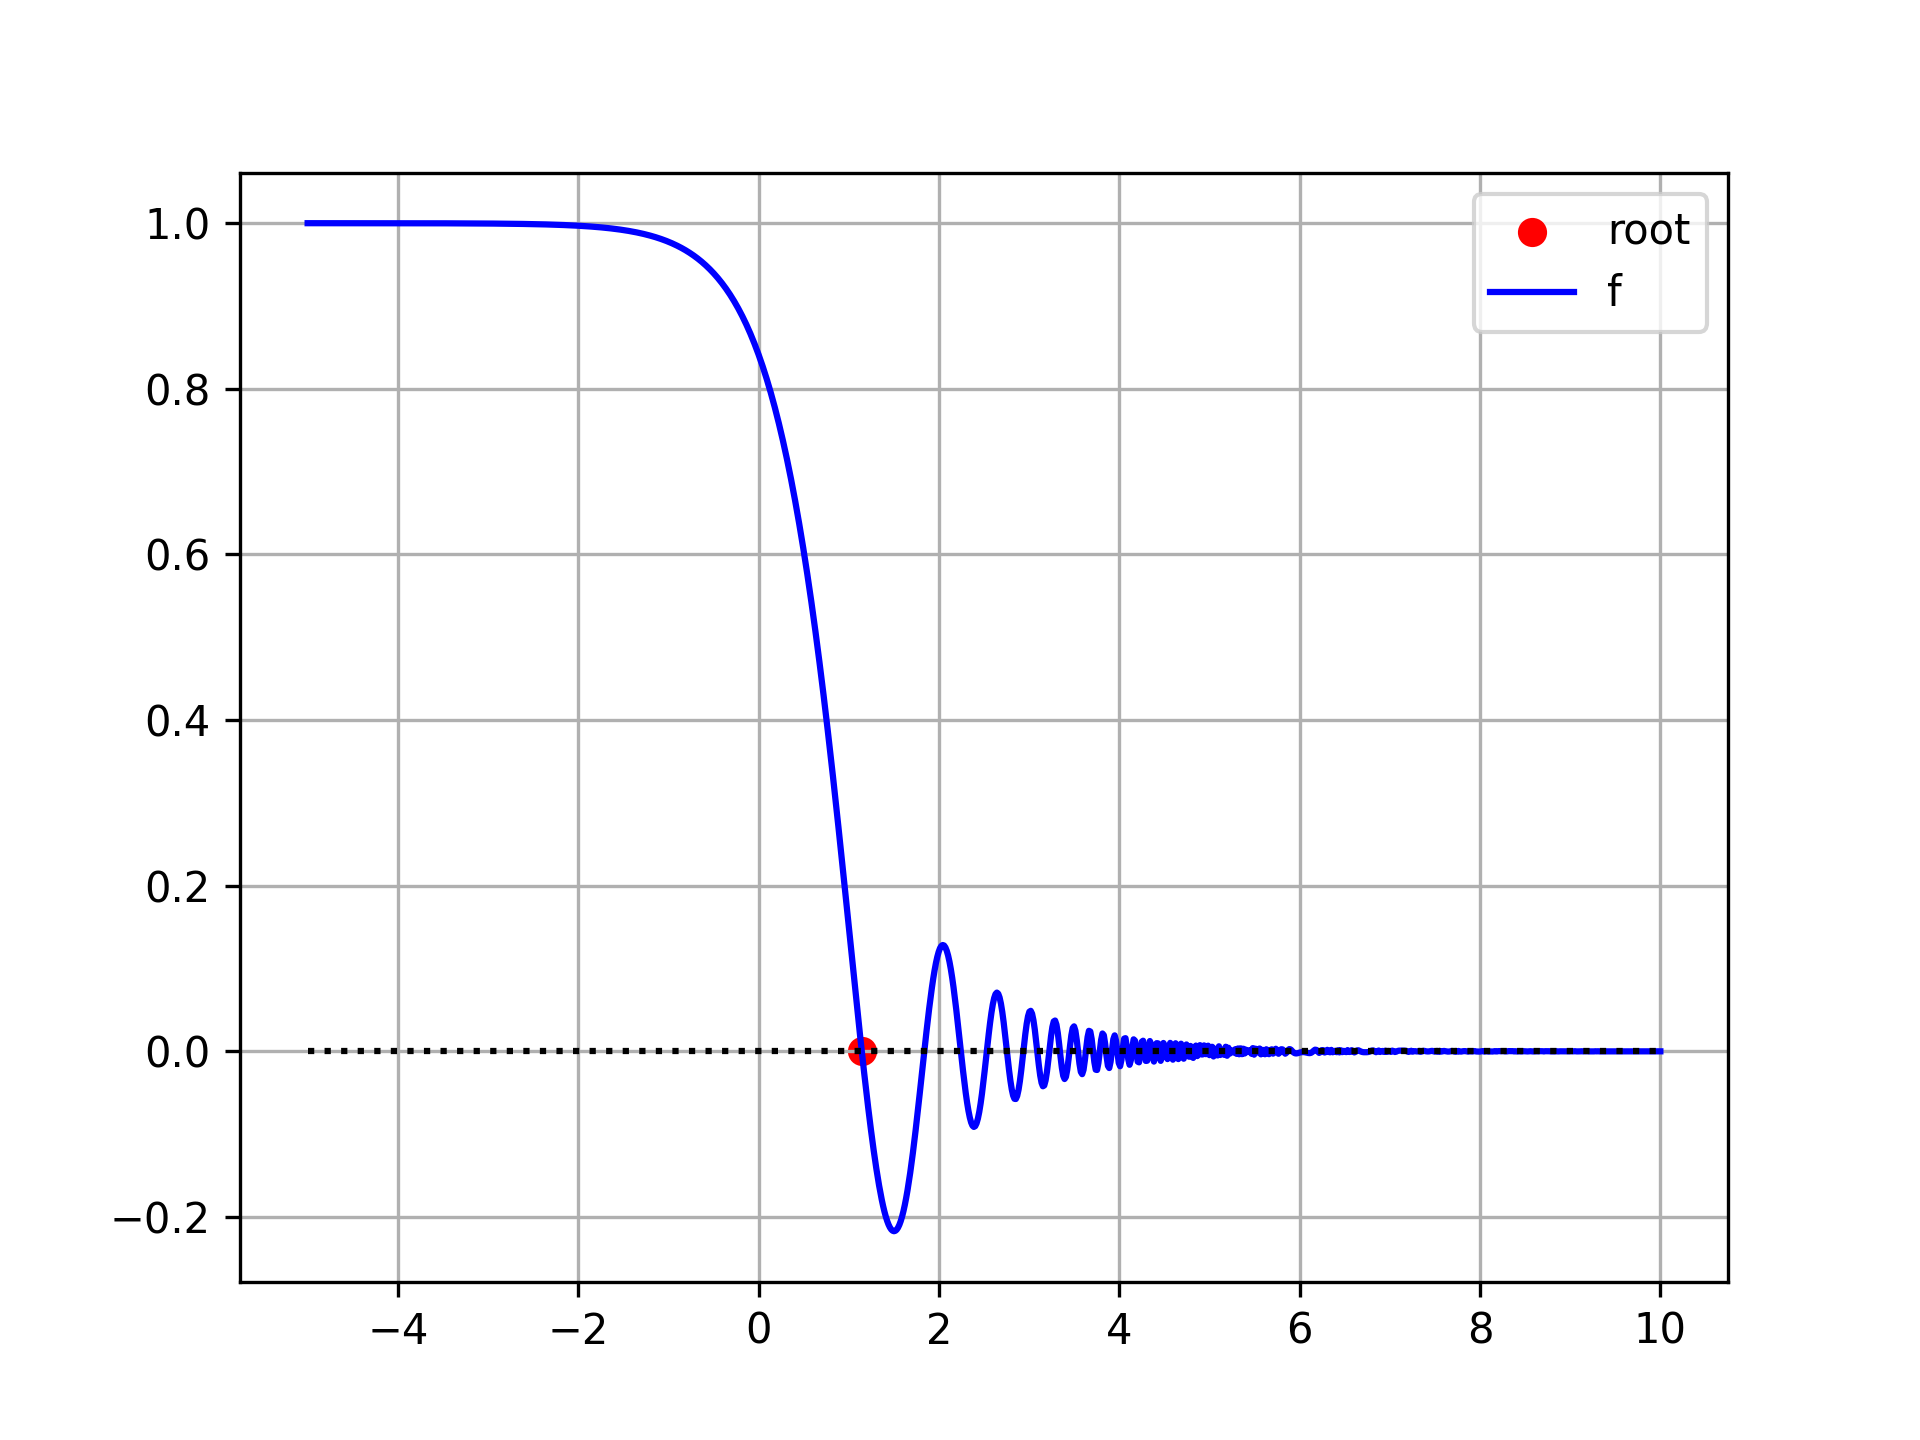
\includegraphics[scale=0.8]{./plots/ffull}
  \caption{A plot of $f$ and its root, on a larger interval}
\end{figure}

\subsubsection{svg - matplotlib}

\begin{figure}[h]
  \centering
  %\includesvg{./plots/svg/ffull.svg}
  \caption{An SVG plot of $f$ and its root, on a larger interval}
\end{figure}

\subsubsection{tikz - pgfplots}


The following TikZ plot looks a little rough if number of samples
is too low. What do you notice when you use 100 samples?

\begin{figure}[h]
  \centering
  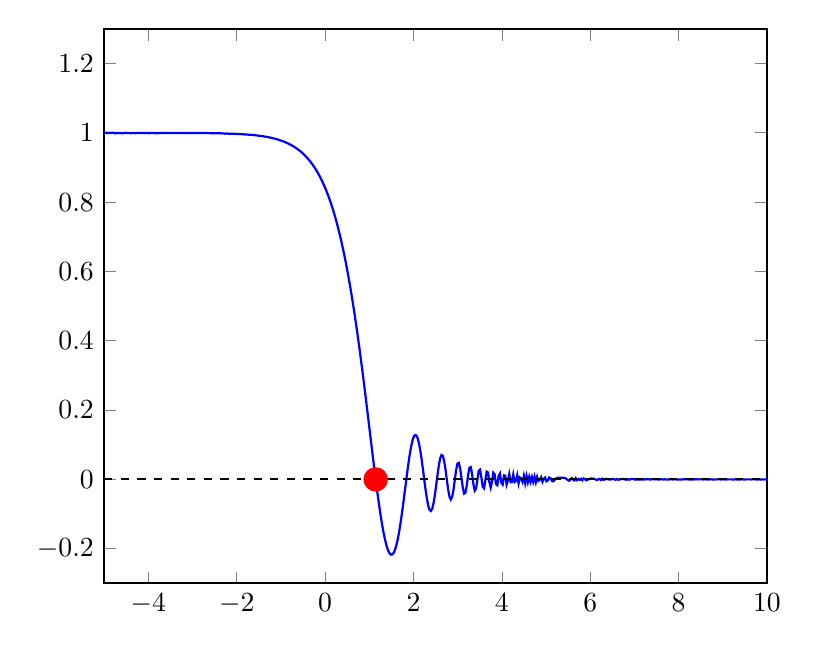
\begin{tikzpicture}
    \begin{axis}[
      samples=500,
      xmin=-5, xmax=10,
      ymin=-0.3, ymax=1.3,
      axis lines=box,
      style=thick,
    ]
    \addplot[domain=-5:10, color=blue]{e^(-x) * sin(deg(e^x))};
    \draw[dashed] (-5,0)--(10,0);
    % plot a point at the root
    \addplot[only marks, mark=*, mark size=4pt, color=red] coordinates {(ln(pi), 0)};
    \end{axis}
  \end{tikzpicture}
  \caption{A TikZ plot of $f$ and its root, on a larger interval}
\end{figure}



\end{document}